%Не забыть:
%--------------------------------------
%Вставить колонтитулы, поменять название на титульнике



%--------------------------------------

\documentclass[a4paper, 12pt]{article} 

%--------------------------------------
%Russian-specific packages
%--------------------------------------
%\usepackage[warn]{mathtext}
\usepackage[T2A]{fontenc}
\usepackage[utf8]{inputenc}
\usepackage[english,russian]{babel}
\usepackage[intlimits]{amsmath}
\usepackage{esint}
%--------------------------------------
%Hyphenation rules
%--------------------------------------
\usepackage{hyphenat}
\hyphenation{ма-те-ма-ти-ка вос-ста-нав-ли-вать}
%--------------------------------------
%Packages
%--------------------------------------
\usepackage{amsmath}
\usepackage{amssymb}
\usepackage{amsfonts}
\usepackage{amsthm}
\usepackage{latexsym}
\usepackage{mathtools}
\usepackage{epstopdf}
\usepackage{etoolbox}%Булевые операторы
\usepackage{extsizes}%Выставление произвольного шрифта в \documentclass
\usepackage{geometry}%Разметка листа
\usepackage{indentfirst}
\usepackage{wrapfig}%Создание обтекаемых текстом объектов
\usepackage{fancyhdr}%Создание колонтитулов
\usepackage{setspace}%Настройка интерлиньяжа
\usepackage{lastpage}%Вывод номера последней страницы в документе, \lastpage
\usepackage{soul}%Изменение параметров начертания
\usepackage{hyperref}%Две строчки с настройкой гиперссылок внутри получаеммого
\usepackage[usenames,dvipsnames,svgnames,table,rgb]{xcolor}% pdf-документа
\usepackage{multicol}%Позволяет писать текст в несколько колонок
\usepackage{cite}%Работа с библиографией
\usepackage{subfigure}% Человеческая вставка нескольких картинок
\usepackage{tikz}%Рисование рисунков
\usepackage{float}
% Для картинок Моти
\usepackage{misccorr}
\usepackage{lscape}
\usepackage{cmap}


\usepackage{graphicx,xcolor}
\graphicspath{{Pictures/}}
\DeclareGraphicsExtensions{.pdf,.png,.jpg}

%----------------------------------------
%Список окружений
%----------------------------------------
\newenvironment {theor}[2]
{\smallskip \par \textbf{#1.} \textit{#2}  \par $\blacktriangleleft$}
{\flushright{$\blacktriangleright$} \medskip \par} %лемма/теорема с доказательством
\newenvironment {proofn}
{\par $\blacktriangleleft$}
{$\blacktriangleright$ \par} %доказательство
%----------------------------------------
%Список команд
%----------------------------------------



\newcommand{\grad}
{\mathop{\mathrm{grad}}\nolimits} %градиент

\newcommand{\diver}
{\mathop{\mathrm{div}}\nolimits} %дивергенция

\newcommand{\Def}[1]
{\underline{\textbf{#1}}} %определение

\newcommand{\RN}[1]
{\MakeUppercase{\romannumeral #1}} %римские цифры

\newcommand {\theornp}[2]
{\textbf{#1.} \textit{ #2} \par} %Написание леммы/теоремы без доказательства

\newcommand{\qrq}
{\ensuremath{\quad \Rightarrow \quad}} %Человеческий знак следствия

\newcommand{\qlrq}
{\ensuremath{\quad \Leftrightarrow \quad}} %Человеческий знак равносильности

\renewcommand{\phi}{\varphi} %Нормальный знак фи

\newcommand{\me}
{\ensuremath{\mathbb{E}}}

\newcommand{\md}
{\ensuremath{\mathbb{D}}}



%\renewcommand{\vec}{\overline}




%----------------------------------------
%Разметка листа
%----------------------------------------
\geometry{top = 3cm}
\geometry{bottom = 2cm}
\geometry{left = 0.7cm}
\geometry{right = 0.7cm}
%----------------------------------------
%Колонтитулы
%----------------------------------------
\pagestyle{fancy}%Создание колонтитулов
\fancyhead{}
%\fancyfoot{}
\fancyhead[C]{\textsc{Геометрическая оптика}}%Вставить колонтитул сюда
%----------------------------------------
%Интерлиньяж (расстояния между строчками)
%----------------------------------------
%\onehalfspacing -- интерлиньяж 1.5
%\doublespacing -- интерлиньяж 2
%----------------------------------------
%Настройка гиперссылок
%----------------------------------------
\hypersetup{				% Гиперссылки
	unicode=true,           % русские буквы в раздела PDF
	pdftitle={Заголовок},   % Заголовок
	pdfauthor={Автор},      % Автор
	pdfsubject={Тема},      % Тема
	pdfcreator={Создатель}, % Создатель
	pdfproducer={Производитель}, % Производитель
	pdfkeywords={keyword1} {key2} {key3}, % Ключевые слова
	colorlinks=true,       	% false: ссылки в рамках; true: цветные ссылки
	linkcolor=blue,          % внутренние ссылки
	citecolor=blue,        % на библиографию
	filecolor=magenta,      % на файлы
	urlcolor=cyan           % на URL
}
%----------------------------------------
%Работа с библиографией (как бич)
%----------------------------------------
\renewcommand{\refname}{Список литературы}%Изменение названия списка литературы для article
%\renewcommand{\bibname}{Список литературы}%Изменение названия списка литературы для book и report
%----------------------------------------
\begin{document}
\begin{titlepage}
\begin{center}
\textsc{Национальный исследовательский университет "Высшая школа экономики"\\[5mm]
Факультет Физики}

\vfill

\textbf{ОТЧЁТ ПО ЛАБОРАТОРНОЙ РАБОТЕ \\[3mm]
"ГЕОМЕТРИЧЕСКАЯ ОПТИКА"\\[3mm]
по курсу "Оптика"
\\[20mm]
}
\end{center}

\hfill
\begin{minipage}{.5\textwidth}
Выполнила:\\[2mm] 
Фазлиахметова Олеся Камилевна\\
БФЗ193\\
2 курс\\[5mm]

Проверила:\\[2mm] 
Готовко С. К. 
\end{minipage}%
\vfill
\begin{center}
 Москва\\
 \today
\end{center}
\end{titlepage}



\tableofcontents

\newpage

\section{Цели работы}

Перед началом работы были поставлены следующие задачи:

\begin{enumerate}
	
	\item Ознакомиться с базовыми оптическими приборами, а также некоторыми методами установки фокусных расстояний линз и оптических систем. 
	
	\item Определить фокусное расстояние плоской положительной линзы различными способами.
	
	\item Определить фокусное расстояние оптической системы с помощью метода Аббе.
	
	\item Определить фокусное расстояние и положение главных плоскостей системы линз.
	
	\item Определить угловое увеличение телескопа.
\end{enumerate}

\section{Определение фокусного расстояния плоской положительной линзы}

Определить фокусное расстояние можно как минимум двумя способами, которые будут приведены ниже.

\subsection{Определение фокусного расстояния с помощью зеркала}

Если расстояние между линзой и объектом будет в точности равно фокусному расстоянию, то изображение объекта будет располагаться на бесконечности. Если за линзой расположить плоское зеркало, то лучи, прошедшие сквозь линзу, отразятся от зеркала и, вновь пройдя сквозь линзу, сформируют перевернутое изображение объекта без увеличения в фокальной плоскости, т.е. в плоскости, в которой расположен объект. Схема представлена на  Рис. \ref{fig:1_1}.

Для того, чтобы было проще определить, что изображение оказалось равновеликим, предмет был такой формы, чтобы его перевернутое равновеликое изображение дополняло его до круга.

Ход работы заключался в следующем: мы собрали установку (см.  Рис. \ref{fig:1_1}) , провели юстировку. Двигали линзу L вдоль оптической скамьи, пока не получили четкое (и равное по размеру с объектом) перевернутое изображение объекта на пластине P. Провели измерение.

Для верности линза была перевернута другой стороной и поставлена в необходимое положение еще раз.

В результате шести измерений были получены следующие значения:

\begin{center}
	\begin{tabular}[H]{|c|c|}
		\hline
		№ измерения & Фокусное расстояние, мм \\
		\hline
		1 & $145 \pm 0.5$ \\
		\hline
		2 & $148 \pm 0.5$ \\
		\hline
		3 & $150 \pm 0.5$ \\
		\hline
		\multicolumn{2}{|c|} {Поворот на 180$^\circ$ }\\
		\hline
		4 & $145 \pm 0.5$ \\
		\hline
		5 & $150 \pm 0.5$ \\
		\hline
		6 & $150 \pm 0.5$ \\
		\hline
	\end{tabular}
\end{center}

Таким образом, усреднив полученные значения, получаем:

\begin{equation*}
	F = 148 \pm 2 \text{ мм}
\end{equation*}


\begin{figure}[H]
	\centering
	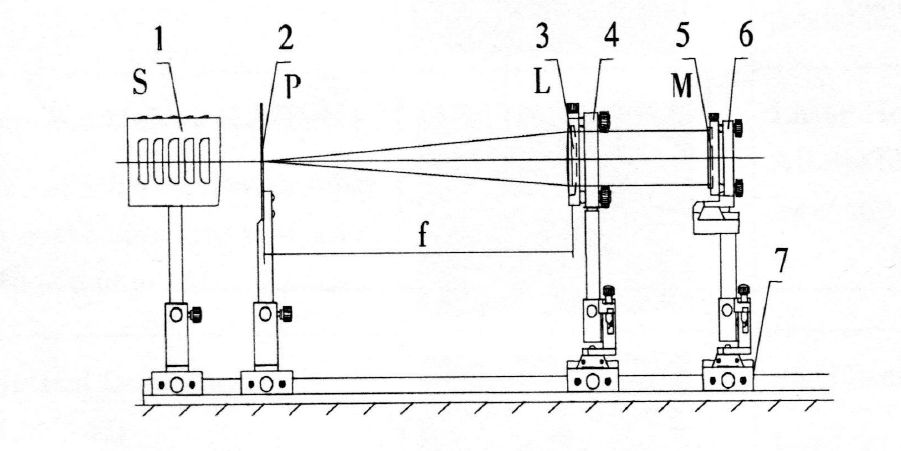
\includegraphics[width=0.8\linewidth]{1}
	\caption{Схема расположения оптических элементов в опыте по определению фокусного расстояния линзы с использованием плоского зеркала. На рисунке изображены следующие элементы: 1~-- осветитель S; 2~-- объект P (LMP-141); 3~-- собирающая линза L ($f=150$ мм); 4, 6~-- двухосевой держатель оптических элементов (LMP-07); 5~-- плоское зеркало М}
	\label{fig:1_1}
\end{figure}

\subsection{Определение фокусного расстояния с помощью экрана}

Этот способ основывается на том, что в случае, когда расстояние от предмета до экрана превышает $4F$, появляется два положения линзы, в которых получается четкое изображение предмета на экране. (в одном случае уменьшенное, в другом -- увеличенное). Из соображений симметрии ясно, что $a_1=a_2'$ и $a_2=a_1'$. Схема опыта представлена на Рис. \ref{fig:1_2}

Пусть  $f$ --- расстояние от линзы до изображения, $L$ --- расстояние между линзой и изображением (экраном).  Пусть расстояние между положениями изображения $l$. Тогда:

\begin{align*}
	a_1 &= \frac{L - l}{2} \\
	a_2 &= \frac{L + l}{2}
\end{align*}

\begin{figure}[H]
	\centering
	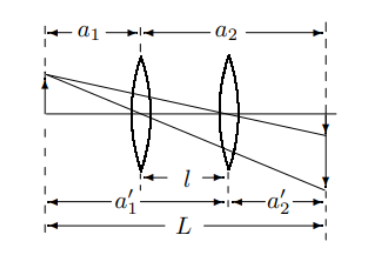
\includegraphics[width=0.4\linewidth]{3}
	\caption{Измерение фокусного расстояния тонкой положительной линзы}
	\label{fig:1_3}
\end{figure}

С учетом формулы тонкой линзы, получим:

\begin{equation}
	F = \frac{L^2 - l^2}{4L}
\end{equation}

Таким образом, необходимо определить необходимую сдвижку линзы $l$ из первого положения, в котором появляется четкое изображение предмета, до второго при заданном $L$. В ходе работы мы перемещали вдоль оптической скамьи линзу, пока не нашли четкое изображение объекта P на экране H. 

В ходе эксперимента были получены следующие результаты:

\begin{center}
	\begin{tabular}{|c|c|c|c|}
		\hline
		№ серии & $L$, мм & $l$, мм & $F$, мм  \\
		\hline
		1 & $650 \pm 0.5$ & $195 \pm 0.5$ & $148 \pm 0.5$  \\
		\hline
		2 & $700 \pm 0.5$ & $273 \pm 0.5$ & $149 \pm 0.5$ \\
		\hline
		3 & $800 \pm 0.5$ & $399 \pm 0.5$ & $151 \pm 0.5$  \\
		\hline
		\multicolumn{4}{|c|} {Поворот на 180$^\circ$ }\\
		\hline
		1 & $700 \pm 0.5$ & $269 \pm 0.5$ & $149.2 \pm 0.5$  \\
		\hline
		2 & $650 \pm 0.5$ & $195 \pm 0.5$ & $147.9 \pm 0.5$ \\
		\hline
		3 & $850 \pm 0.5$ & $469 \pm 0.5$ & $148 \pm 0.5$  \\
		\hline
	\end{tabular}
\end{center}

После усреднения всех полученных фокусных расстояний, получаем: 

\begin{equation*}
	F = 148.85 \pm 1.21 \text{ мм}
\end{equation*}

\begin{figure}[H]
	\centering
	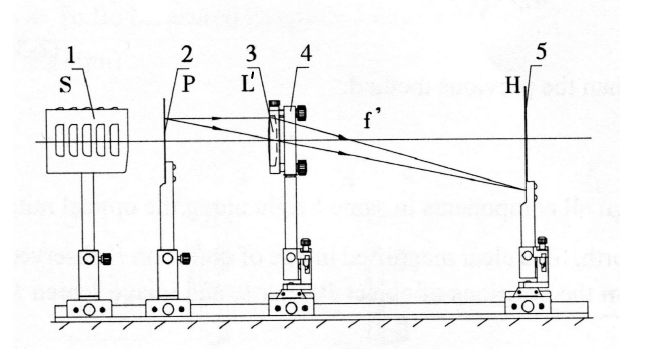
\includegraphics[width=0.7\linewidth]{2}
	\caption{Схема расположения оптических элементов в опыте по определению фокусного расстояния линзы с использованием экрана. На рисунке изображены следующие элементы: 1~-- осветитель S; 2~-- объект P (LMP-14); 3~-- собирающая линза L' ($f=150$ мм); 4~-- двухосевой держатель оптических элементов (LMP-07); 5 – экран Н}
	\label{fig:1_2}
\end{figure}

\section{Определение фокусного расстояние оптической системы с помощью метода Аббе}

Фокусное расстояние оптической системы может быть измерено также с помощью метода Аббе. Получим расчетную формулу.

Предположим, что линейный размер предмета равен $y$, а находится он на расстоянии $x_1$ от главного фокуса $F$ положительной оптической системы. Изображение предмета в таком случае имеет размер $y_1$, а линейное увеличение равно $\beta_1 = y_1 / y = F / x$. Если же теперь передвинуть предмет на небольшое расстояние $\Delta x$, то увеличение изменится и станет равным $\beta_2 = y_2 / y = F / x$. В таком случае, легко получить:

\begin{equation}
	F = \frac{\Delta x}{\frac{1}{\beta_1} - \frac{1}{\beta_2}}
	\label{eq:1}
\end{equation}

Таким образом, необходимо определить линейное увеличение $\beta_1$ в одном положении линзы, и линейное увеличение $\beta_2$ в сдвинутом относительно первого на $\Delta x$. Схема опыта представлена на Рис. \ref{fig:2}.

В результате экспериментов были полученные следующие данные:

\begin{center}
	\begin{tabular}{|c|c|c|c|c|}
		\hline
		 № & $\beta_1$ & $\Delta x$, мм & $\beta_2$ & F, мм \\
		\hline
		1 & 1.2 & 10 & $\frac 5 3$ & 42.8 \\
		\hline
		2 & $\frac 4 3$ & 10 & 1 & 40\\
		\hline
		3 & 1.1 & 11 & 1.5 & 33 \\
		\hline
	\end{tabular}
\end{center}

Тогда, с учетом формулы (\ref{eq:1}), получаем значение фокусного расстояния:

\begin{equation*} 
	F = 38.6 \pm 4.1 \text{ мм}
\end{equation*}

\begin{figure}[H]
	\centering
	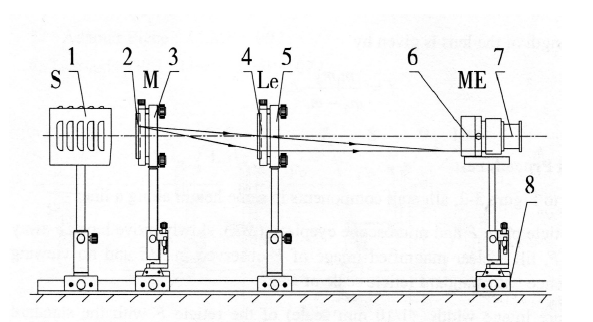
\includegraphics[width=0.7\linewidth]{4}
	\caption{Схема расположения оптических элементов в опыте по определению фокусного расстояния линзы с помощью метода Аббе. На рисунке изображены следующие элементы: 1~-- осветитель S; 2~-- слайд с делениями M (Reticle); 3~-- держатель бипризм (LMP-41); 4~-- линза Le ($f=35$ мм); 5~-- двухосевой держатель оптических элементов (LMP-07); 6~-- окуляр микроскопа МЕ; 7~-- держатель микроскопа (LMP-09)}
	\label{fig:2}
\end{figure}

\section{Определение фокусного расстояния и положения главных плоскостей системы линз}

Рассмотрим оптическую систему, которая состоит из двух центрированных собирающих линз, расположенных на известном расстоянии друг от друга. 

Если система состоит из двух собирающих линз, то фокусное расстояние системы можно рассчитать следующим образом:

\begin{equation}
	\frac{1}{F} = \frac{1}{F_1} + \frac{1}{F_2} - \frac{l_{12}}{F_1 F_2}
	\label{eq:2}
\end{equation}

Здесь $l_{12} = 40 \pm 0.5$ мм --- расстояние между линзами.

План работы: собрали установку (Рис. \ref{fig:3_1}), установили линзу $L_0$ на фокусном расстроении от объекта, получили изображение на бесконечности. За $L_0$ расположили систему линз $L_1-L_2$, расстояние между которыми  $l_{12}$. Двигали экран вдоль оптической оси и находили четкое изображение (экран в этом случае находится в задней фокальной плоскости системы линз). Повернули обе линзы и повторили действие.  В ходе эксперимента было определено взаимное положение фокальных плоскостей относительно оптической системы, представленное на Рис. \ref{fig:3_2}.

Полученный результат:

\begin{center}
	\begin{tabular}{|c|c|}
		\hline
		№ опыта & Фокальная плоскость F, мм\\
		\hline
		1 & 121 $\pm 0.5$  \\
		\hline
		2 & 118 $ \pm 0.5$ \\
		\hline
	\end{tabular}
\end{center}

После усреднения получим:
$F = 119.5\pm 1.5$ мм

Теперь определим фокусное расстояние с помощью метода Аббе. Схема опыта представлена на рисунке \ref{fig:3_1}. После эксперимента были получены следующие данные:

\begin{center}
	\begin{tabular}{|c|c|c|}
		\hline
		$\beta_1$ & $\Delta x$, мм & $\beta_2$ \\
		\hline
		1.2 & 20 & 1.5 \\
		\hline
	\end{tabular}
\end{center}

Тогда по формуле (\ref{eq:1}) получаем:

\begin{equation*}
	F_{abbe} = 120 \text{ мм}
\end{equation*}

Поскольку фокусные расстояния каждой из линз известны (написаны на их ободе) и равны $F_1 = 190 \text{ мм}$ и $F_2 = 300 \text{ мм}$, по формуле же (\ref{eq:2}), которая выведена для конкретной системы, получим:

\begin{equation*}
	F_{theor} = 126 \text{ мм}
\end{equation*}


\begin{figure}[H]
	\centering
	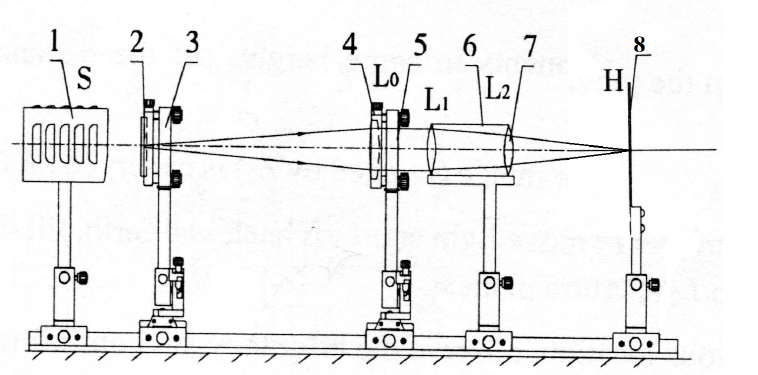
\includegraphics[width=0.7\linewidth]{5}
	\caption{Схема расположения оптических элементов в опыте по определению фокусного расстояния оптической системы с помощью метода Аббе. На рисунке изображены следующие элементы: 1~-- осветитель S; 2~-- слайд с линейкой (Millimetre Ruler); 3~-- держатель бипризм (LMP-41); 4~-- линза L0 ($f=150$ мм); 5~-- двухосевой держатель оптических элементов (LMP-07); 6~-- оптическая система, состоящая из линз L1 ($f=190$ мм) и L2 ($f=300$~мм); 7~-- держатель группы линз (LMP-28); 8~-- экран Н (LMP-13)}
	\label{fig:3_1}
\end{figure}

\begin{figure}[H]
	\centering
	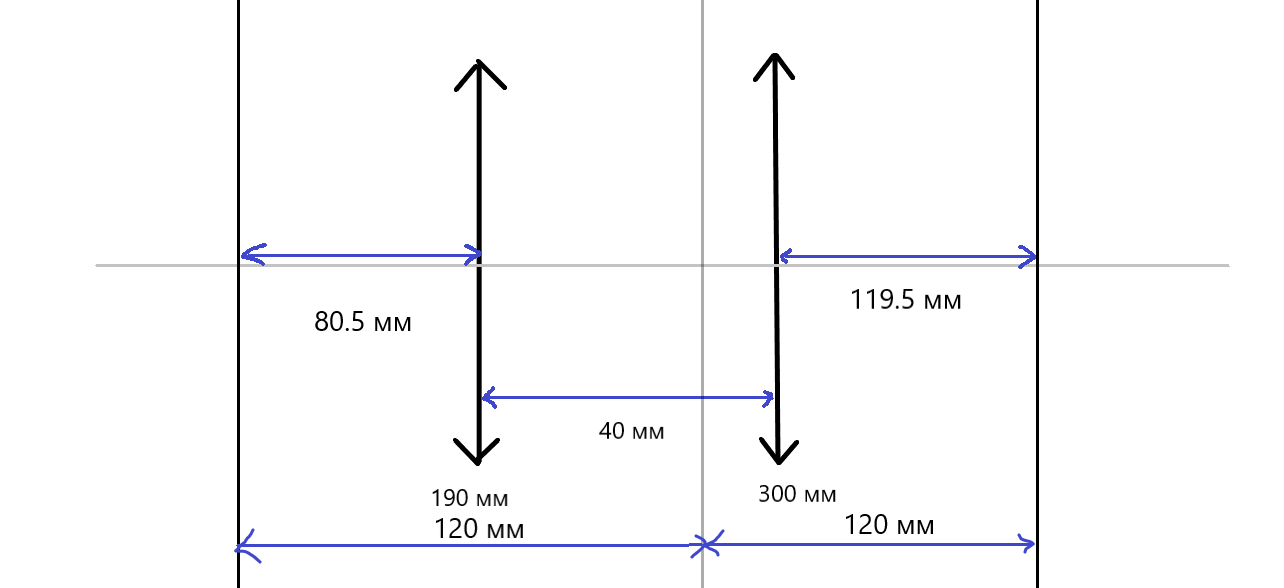
\includegraphics[width=\linewidth]{6}
	\caption{Взаимное расположение фокальных плоскостей оптической системы относительно линз}
	\label{fig:3_2}
\end{figure}


\section{Определение углового увеличения телескопа}

В настоящей работе изучается модель астрономической зрительной
трубы. Этот оптический прибор состоит из двух основных частей: объектива
— линзы, обращённой к объекту, и окуляра — линзы, обращённой к
наблюдателю. Объектив, в качестве которого используется положительная
линза, создаёт действительное изображение предмета. Это изображение
рассматривается глазом через окуляр. Ход лучей в астрономической
зрительной трубе (трубе Кеплера) представлен на Рис. \ref{fig:4_1}.

\begin{figure}[H]
	\centering
	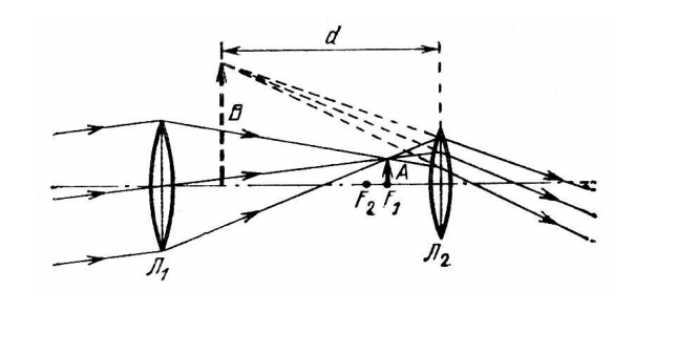
\includegraphics[width=0.6\linewidth]{7}
	\caption{Ход лучей в трубе Кеплера}
	\label{fig:4_1}
\end{figure}

Для определения углового увеличения телескопа было сделано следующее.

После слайда-линейки, который выступает в роли объекта, была установлена на ее фокусном расстоянии линза. Это позволяет получить параллельный пучок света, с которым обычно и работают при использовании телескопа. После этого с помощью зрительной трубы было определено число штрихов на линейке $N_1 = 8$, которые укладывались в поле зрения трубы. Затем после линзы была установлена собранная труба Кеплера ($F_1 = 190 \text{ мм, } F_2 = 105 \text{ мм}$) и данная операция была проделана еще раз, с получившимся $N_2 = 4$.

Угловым увеличением в таком случае по определению будет являться:

\begin{equation}
	\gamma_N = \frac{N_1}{N_2} = 2
\end{equation}

С другой стороны, угловое увеличение телекопа равно  отношению фокусов объектива и окуляра:

\begin{equation*}
	\gamma_f = \frac{F_1}{F_2} = 1.81
\end{equation*}


\section{Вывод}

\begin{enumerate}
	\item Ознакомление с приборами и методами определения фокуса было проведено.
	
	\item Было установлено фокусное расстояние линзы с помощью двух методов: с использованием зеркала и с использованием экрана, которые дали результаты, неплохо сходящиеся с реальностью и друг с другом: $F = 148\pm 2$ мм для метода с зеркалом и $F = 148.85 \pm 1.21$ мм для метода с использованием экрана. 
	
	\item С помощью метода Аббе было установлено фокусное расстояние линзы $F = 38.6\pm 4.1$ мм.
	
	\item  Для имеющейся системы из двух собирающих линз было определено ее фокусное расстояние, оказавшееся равным $F_{abbe} = 120 \text{ мм}$ и $F = 119.5\pm 1.5 \text{ мм} $ по данным эксперимента и $F_{theor} = 126 \text{ мм}$ по предсказаниям теории. Было также получено расположение главных плоскостей системы относительное ее центра, представленное на рисунке \ref{fig:3_2}. 
	
	\item Было определено угловое увеличение телескопа, которое оказалось равным $\gamma_N = 2$ из эксперимента и $\gamma_f = 1.81$ из теории. 
\end{enumerate}





\end{document}